\documentclass[nofonts]{ctexrep}
\setCJKmainfont[ItalicFont={AR PL UKai CN}]{AR PL UMing CN} %设置中文默认字体
\setCJKsansfont{WenQuanYi Micro Hei} %设置文泉驿正黑字体作为中文无衬线字体
\setCJKmonofont{WenQuanYi Micro Hei Mono} %设置文泉驿等宽正黑字体作为中文打字机字体

\usepackage{comment}
\usepackage[linesnumbered]{algorithm2e}
\usepackage{graphicx}
\usepackage{listings}
\usepackage{multirow}
\usepackage{url}
\usepackage{color}
\usepackage{listing}
\usepackage{xspace}
\newcommand{\code}[1]{\texttt{\footnotesize #1}}
\newcommand{\todo}[1]{{\color{red} \bf \{TODO: {#1}\}}}

\def\modify#1#2#3{{\small\underline{\sf{#1}}:} {\color{red}{\small #2}}
{{\color{red}\mbox{$\Rightarrow$}}} {\color{blue}{#3}}}
%\renewcommand{\modify}[3]{{#3}}

\newcommand{\yxmodify}[2]{\modify{Yingfei}{#1}{#2}}

\newcommand\mymargin[1]{\marginpar{{\flushleft\textsc\footnotesize {#1}}}}
\newcommand\yxmargin[1]{\mymargin{YX:\;#1}}

\newcommand{\figref}[1]{Figure~\ref{#1}}
\newcommand{\eqnref}[1]{violation~\eqref{#1}}
\newcommand{\secref}[1]{Section~\ref{#1}}
\newcommand{\tblref}[1]{Table~\ref{#1}} 
\newcommand{\algref}[1]{Algorithm~\ref{#1}} 
\newcommand{\smalltitle}[1]{{\smallskip \noindent \bf  {#1}.\ }}
\newcommand{\smalltitlecolon}[1]{{\smallskip \noindent \bf  {#1}:\ }}

\newtheorem{property}{Property}

\newcommand{\yxmodifyok}[2]{#2}

\newcommand{\mycomment}[2]{{\small\color{magenta}\underline{\sf{#1}}:} {\color{magenta}{\small #2}}}
\newcommand{\yxcomment}[1]{\mycomment{Yingfei}{#1}}

% \renewcommand{\yxcomment}[1]{}
% \renewcommand{\yxmodify}[2]{#2}
\usepackage{amsmath,amssymb}
\usepackage{graphicx}
\usepackage{bm}
\usepackage[linesnumbered]{algorithm2e}
%\usepackage{titleps}
%\usepackage{times}
\usepackage{titlesec}
\usepackage[labelsep=none]{caption, subcaption}
%\setlength{\itemsep}{5mm}
\usepackage{indentfirst}
\usepackage{enumerate}
%\usepackage{biblatex}
%\usepackage{float}
%\newcommand{\myfontsize}{\fontsize{13pt}{\baselineskip}\selectfont}
\renewcommand{\bibname}{参考文献} 

\usepackage{geometry}
\geometry{left=3.5cm,right=3.5cm,top=4cm,bottom=4cm}

%\titleformat{\chapter}[display] {\Huge\bfseries} {Chapter \thechapter} {1pc} {\vspace{1pc} \Huge}
%\titleformat*{\section}{\LARGE\bf}
%\titleformat*{\subsection}{\Large\bf}
%\titleformat*{\subsubsection}{\large\bf}
%\setmainfont{Times New Roman}
%\captionsetup{font={scriptsize}}
%\captionsetup{labelfont={scriptsize}}




\usepackage{fancyhdr}
\pagestyle{fancy}
\fancyhf{}
%\fancyhead[EL, OL]{\leftmark}
\fancyhead[ER, OR]{\leftmark}
\fancyfoot[C]{\thepage}
\renewcommand{\chaptermark}[1]{\markboth{#1}{}}
\CTEXsetup[name={,}]{chapter}

\newtheorem{lemma}{引理}
\newtheorem{proof}{证明}
\newtheorem{corollary}{结论}
\newtheorem{theorem}{定理}

\begin{document}
%\bibliographystyle{plain}
\begin{titlepage}
\begin{center}
\LARGE

\vspace{20mm}
北京大学信息科学技术学院\\
\vspace{5mm}
本科生毕业论文\\
\vspace{70mm}
\textbf{\huge 动态变异测试:设计与实现}\\
\vspace{20mm}
1200012741\\
史杨勍惟\\
\vspace{20mm}
指导老师:熊英飞\\
\vspace{10mm}
(\today)
\end{center}
\end{titlepage}

%\newpage
%\newpage
\renewcommand{\baselinestretch}{1.5}
%\Large

% Done by 04/25
\large
\chapter*{摘要}
变异测试是一种在通过细节改变源代码的软件测试方法,用来帮助测试者评估测试集的质量。变异测试一个很大的瓶颈在于其可扩展性。研究人员已经提出了各种不同的变异测试的加速技术,例如移除冗余的变异体等。然而,这些技术都是静态的,所以无法消除在变异体执行过程中的冗余部分。

本论文的目标是设计一个动态变异测试技术:在变异测试的执行过程中对变异体进行分析,仅在变异体产生新的系统状态的时刻创建新进程来执行变异体。基于此技术,本论文在LLVM的框架上实现了一个C语言变异测试的加速工具AccMut,并将此工具与现有的加速技术进行了对比和验证。实验表明动态变异测试的加速效果显著,加速比是Major Framework(目前最快的静态变异测试加速技术)的X倍。\\

\textbf{关键词:} 变异测试,变异算子,变异体,动态分析, 抽象模型
\chapter*{Abstract}
Mutation analysis is used to help evaluating the quality of existing software tests by modifying a program in small ways. One important bottleneck of mutation analysis is its scability. Researches have proposed different techniques to accelerate the mutation analysis, such as removing redundant computations in mutation analysis. However, all these techniques are static, and thus cannot remove redundancy that occurs in part of mutant execution. 


The purpose of this thesis is to design a technique to accelerate the mutation analysis dynamically, which analyzes the mutants during the execution of the program and forks the execution only when a mutant leads to a new system state. Based on this techinque, we developed an acceleration tool "AccMut" on C programming language on top of LLVM and compared it with other techniques. Our experiment show that our approach can accelerate mutation analysis significantly, having a speedup up to x.xxX over Major Framework, a state-of-the-art tools of static acceleration. \\

\textbf{Keyword:} mutation analysis, mutation operator, mutant, dynamic analysis, abstract model
\tableofcontents

%\renewcommand{\baselinestretch}{2.0}
%\large

% Done by 04/25
\chapter{引言}
\section{变异测试}
变异测试是一种软件测试方法,也是一种重要的程序分析技术\cite{demillo1978hints,hamlet1977testing}。
图X描述了变异测试的整个流程。给定一个程序,变异测试通过一些预定义的变异算子对程序进行微小的修改,产生一个程序集合。此集合中的每个程序和原程序都有细微的差别,这些程序称之为原程序的变异体。随后变异测试在这个程序集合的所有程序上对已有的测试集数据进行测试,并统计执行过程中的信息和执行结果进行下一步分析。


变异测试的主要用途是帮助测试员评价测试集的质量\cite{jia2011analysis}。按照通常的理解:一个好的测试集能够检测出程序中所有潜在的错误。变异测试就是这个过程的逆向过程:每一个变异体可以看成一个有潜在错误的程序,如果一个测试集在任何一个变异体上都无法通过,那么这个测试集就可以视作是一个好的测试集。变异测试还有其他的用途,例如缺陷定位~\cite{papadakis2012using,moon2014ask,zhang2013injecting}和缺陷修复~\cite{GenProg,PAR,RSRepair,AE}等。

常见的变异算子包括:符号变异(逻辑符号变异,算数符号变异),数值变异,语句级变异(插入或删除一条语句),过程级变异(函数的替换)。变异测试生成的大部分变异体为一阶变异体(即变异体和原程序只有一处不同),有些时候根据需要,变异测试也会生成高阶变异体(即变异体和原程序有几处不同)。
高阶变异测试。

\section{变异测试的瓶颈}
变异测试有一个重要的瓶颈:可扩展性较差。假设一个程序的测试集中有$m$组输入,而变异测试在这个程序上生成了$n$个变异体,那么整个变异测试的执行过程需要在$n\times m$倍的程序执行时间。虽然$m$是固定的,但是当我们对变异算子进行扩展的时候,变异体数量$n$就会随之膨胀,进一步导致整个变异测试的时间就会显著增加。这也是变异测试在实践中只是被小规模采用的原因。

\section{相关工作}
为了解决可扩展性的问题,近年来研究人员已经提出了各种不同的方法来加速变异测试的执行。这些方法可以分为有损加速和无损加速。

\subsection{Weak Mutation}
Weak Mutation\cite{howden1982weak}是一个典型的有损加速技术,Weak Mutation认为只要变异体在某一个测试用例上产生了和原程序不同的系统状态,那么就认为这个这个测试用例无法通过此变异体。这显然是一个有损的方法(因为有些变异体即使产生了不同的系统状态,也不一定会产生错误的结果)。
\subsection{Mutation Sampling}
Mutation Sampling~\cite{wong1995reducing}是另一种有损加速技术,它在所有变异体中选取一些具有代表性的变异体,并且只在这些变异体上进行测试,来减少执行时间。
\subsection{Major Framework}
Major Framework~\cite{just2014efficient}是目前为止最快的无损加速工具。它通过静态分析的方式结合测试集中每组测试用例的数据对程序进行预处理,对剩变异体进行等价类划分。Major Framework按照下面三个标准进行等价类划分:

\begin{itemize}
\item 如果一个测试用例没有覆盖到某个变异体的变异点语句,那么这个变异体就可以认为是和原程序等价的。
\item 如果两个变异体所产生的变异点在同一个复合表达式上,而这个表达式的值是一样的,那么这两个变异体就可以认为是等价的。
\item 如果两个变异体在一个测试用例上在变异点语句上的所有执行结果都相同,那么这两个变异体就可以认为是等价的。
\end{itemize}

划分完成后,Major Framework逐一执行测试用例的每组测试用例。在一个等价类中任意选出一个一个变异体执行该测试用例,而不需要在其他变异体上执行了。这样就每个测试用例就可以节省很多等价的重复执行,节省了时间。

\subsection{Mutation Schemata}
Mutation Schemata从编译时间上加速了变异测试。由于每个变异体都是一个新的程序,所以编译变异体需要大量的时间。Mutation Schemata将所有的变异体整合到了同一个程序上,只编译一次,节省了大量的编译时间。

\subsection{Test Prioritization}
Test Prioritization~\cite{zhang2013faster}针对不同变异体对测试集中的不同测试用例进行了重排,使得变异体尽可能早地被检测出,这样就不用执行测试集中的其他测试用例了。此方法并没有具体工具的实现。


\section{本论文的目标}
以上的加速技术有一个共同的不足:它们都是静态加速的方式。任意给定两个变异体,在发生变异的变异点之前,这两个程序在同一个输入上的执行过程是完全相同的,而静态加速的方法无法消除程序执行过程中(图X的X部分)的冗余部分,导致这个过程被重复执行了两遍。

本论文的目标是设计一个动态变异测技术:在变异测试的执行过程中对变异体进行分析,仅在变异体产生新的系统状态的时刻创建新进程来执行变异体。与静态加速技术不同,此动态变异测试技术从一个包含了所有变异体的程序开始执行,每遇到一个包含了变异体的语句,就对此语句以及所有的变异语句作动态分析,根据分析结果进行等价类划分。当且仅当有新的等价类诞生的时候(表示此变异体集合会产生新的系统状态),原程序会创建一个新的进程,在这个进程中执行新的等价类的变异体。这个方法是无损的,这个方法有以下两个优点:
\begin{itemize}
\item 不同的变异体在变异点之前共享同一个执行过程,从而消除了执行过程中的冗余部分。从而节省了大量的执行时间。
\item 此方法将所有变异整合到了同一个程序中,无需编译多次,这是Mutation Schemata的优点。在动态执行过程中可以根据即时的结果进行等价类的划分,复用等价变异体的执行,这是Major Framework的优点。所以此方法集合了现有的两大静态加速技术,进一步提升了加速比。
\end{itemize}

本论文定义了支持变异测试的抽象模型,并且在这个模型上给出了静态变异测试的算法,设计了动态变异测试的算法。我们在LLVM的框架上实现了一个C语言变异测试的加速工具AccMut,并同时在LLVM的框架上复现了现有的加速工具(Schemata,Major Framework)用来进行横向对比和验证。实验表明动态变异测试技术加速效果显著,加速比是Major Framework(目前最快的静态变异测试加速技术)的X倍。

\section*{说明}
我的本科生科研的课题也是变异测试的加速,本论文和本科生科研论文的主要区别在于等价类划分算法的实现和IO支持上。本科生科研时我采用的等价类划分使用的是复现的Major Framework的划分方法,而本论文则使用的是纯动态的自行设计的等价类划分方法;另一方面,本论文实现的工具已经支持下涉及读写独立的文件IO的程序,而在本科生科研实现的工具中并不支持。在实验的规模上,本论文也超出了本科生科研时后的规模。总的来说,本论文在本科生科研的成果上做了许多扩展和修改工作。

% Done by 04/27 10+
\chapter{方法}
\section{加速原理}
图X描述了我们的动态变异测试技术如何消除执行过程中的冗余过程。图中的每个圆圈代表了一个系统状态,数字相同的圆圈代表了相同的系统状态。箭头代表了在执行一句或者多句语句之后的系统状态的转换过程。在状态2,图中的三个变异体执行了三句不同的语句,是的系统状态转换为了两个不同的系统状态(状态3和状态5)。其中,虽然其中两个变异体(变异体1和变异体3)的语句是不同,但它们产生的结果是相同的,即转换后的系统状态是相同的。这是可能发生的,比如当$a==2$的时候,语句$a+=2$和语句$a*=2$执行后的效果是一样的。在状态3,变异体1和变异体3再次执行了不同的语句,而这次两个变异体执行的语句产生了不同的结果,转换后的系统状态不想同。所以,状态1,状态2,以及之前的一系列状态对于这三个变异体来说是完全相同的,这就导致了冗余的执行过程。同理,状态5以及之前的一系列状态对于变异体1和变异体3来说也是完全一样的,也是冗余的执行过程。根据重复度的不同,我们把冗余的执行过程标注成了黑色的或者是灰色的圆圈。

因为这三个变异体最终产生的系统状态是不同的,所以在它们的执行过程中,只有其中一部分使可以消除的,这就意味着任何静态加速技术无法消除这部分冗余的执行过程。相比之下,动态变异测试技术可以通过在执行过程中创建新进程的方法来复用这部分的重复执行。变异测试的动态执行方法从一个代表了所有变异体的主进程开始执行,如图X。在每个系统状态,我们检查在这个系统状态下所有变异体将要执行的语句。如果所有变异体将要执行的语句是一样的,那么我们就简单地执行这条语句;如果存在不同的可能需要执行的语句,那么我们就对不同的执行过程可能产生的结果进行分析,并且在需要的时刻创建新的进程。在状态2,三个变异体有三个不同的语句需要执行,所以我们需要分析这三条语句可能产生的执行结果。

\begin{figure}[ht]
  \centering
  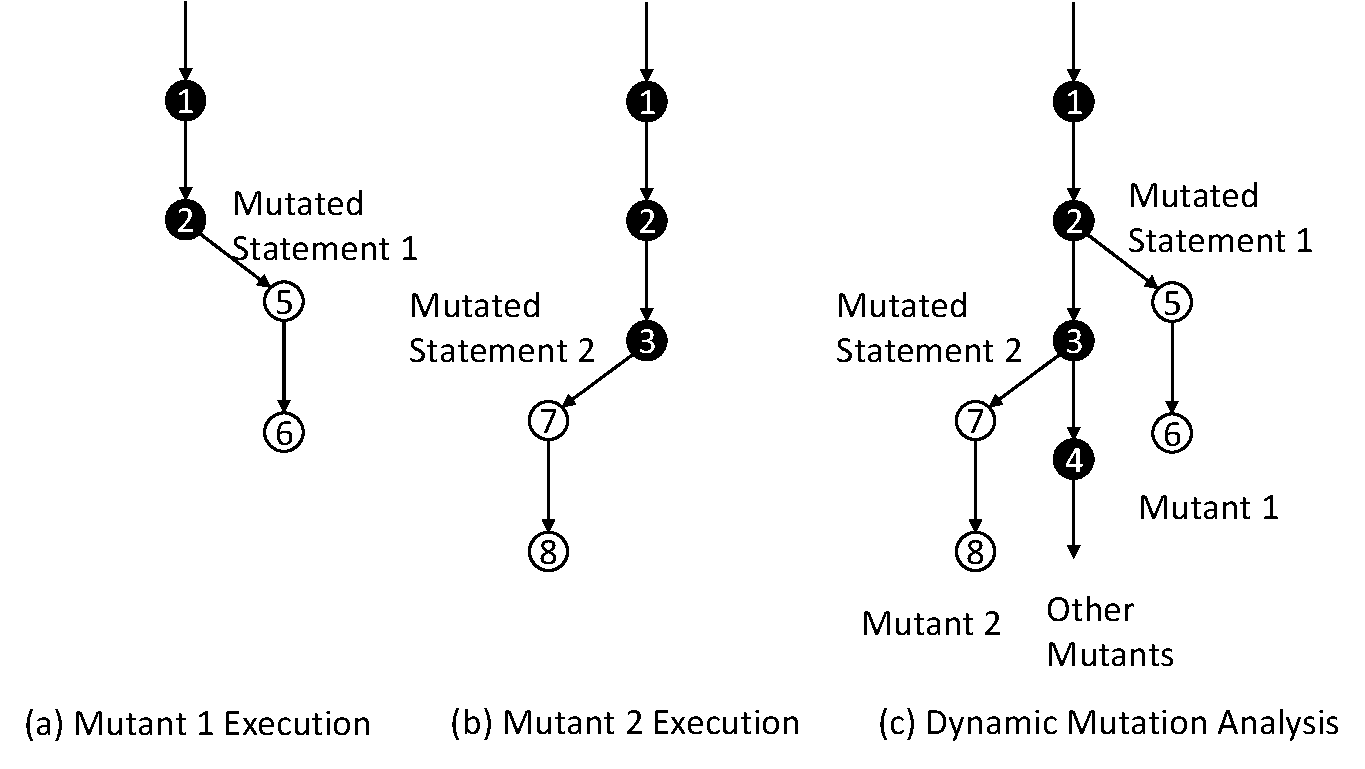
\includegraphics[width=\columnwidth]{figs/redundancy}
  \caption{Dynamic Mutation Analysis with Forking\label{fig:redundancy} }
\end{figure}

分析过程中,我们依次模拟执行每条语句并且收集它们的结果。根据不同地结果,我们将这些变异体划分成不同的等价类。两个变异体在个系统状态是等价的当且仅当这两个变异体在这个系统状态下所需要执行的语句是一样的或者这两个变异体在这个系统状态下所执行的语句产生的结果是一样的。例如,状态2下,变异体1和变异体3虽然执行的语句不一样,但是产生的结果是一样的,那么变异体1和变异体3在状态2下就被认为是等价的,归入同一个等价类。

如果在某个状态下,我们分析并生成了n个等价类(n>1),那么我们就要创建n-1个新进程。每个新创建的进程都代表一个等价类,在这个进程中,我们在其代表的等价类的变异体中任意选取一个语句(在这个系统状态下的)并执行该语句。在这个离子重,在状态2下,我们创建一个子进程代表变异体1和变异体3并执行其中任何一个的语句,进而转换为状态5,到了状态5,此新进程有创建出一个孙子进程代表变异体3,孙子进程执行变异体3的语句转换为状态7,子进程执行变异体1的语句转换为状态6,而原进程在状态2执行变异体2的语句,转换为状态3,进而转换为状态4。

从图X中我们可以看到,状态1之前的转换,状态1到状态2的转换,以及状态2到状态5的转换都只执行了一次,所以不会有冗余的执行过程。


\subsection{相关背景:系统调用fork()}
我们的方法使用系统调用fork()来创建新线程。fork()是POSIX系统中的一个系统调用,在其他操作系统例如Windows,也有fork()系统调用的实现(通过Cygwin支持)。当我们调用fork()函数的时候,系统会创建一个新的子进程,这个子进程与创建它的进程(父进程)具有相同的系统状态(包括虚拟内存空间和栈帧空间)。父进程和子进程最大的区别在于fork()函数的返回值。fork()向子进程返回0,向父进程返回子进程的进程号。我们也是基于这个返回值来确定当前执行的是父进程还是子进程。

POSIX系统调用fork()通过``写时拷贝''机制来实现:当fork()被调用的时候,系统会创建一个新的进城对象并且赋予其一些基本信息,例如进程号等,但是并没有马上从父进程拷贝虚拟内存空间而是与其父进程共享虚拟内存空间。当且仅当某一个进程(父进程或者子进程)的虚拟内存空间发生写操作的时候,系统才会对所写页创建一份新的拷贝,并且更新子进程的页表信息。``写时拷贝''机制被集成到了虚拟内存访问的过程中,所以系统调用fork()本身的执行速度很快,同时被创建的子进程的执行速度和普通进程(不是从另一个进程创建出来的进程)执行速度并没有太大差距。

\section{抽象模型}
\newcommand{\mids}{\ensuremath{I}\xspace}
\newcommand{\execute}{\ensuremath{\mathrm{execute}}\xspace}
\newcommand{\try}{\ensuremath{\mathtt{try}}\xspace}
\newcommand{\apply}{\ensuremath{\mathtt{apply}}\xspace}
\newcommand{\filterv}{\ensuremath{\mathrm{filter\_variants}}\xspace}
\newcommand{\filterm}{\ensuremath{\mathrm{filter\_mutants}}\xspace}
\newcommand{\filterom}{\ensuremath{\mathrm{filter\_out\_mutants}}\xspace}
\newcommand{\VectorSet}{{\tt VectorSet}\xspace}
\newcommand{\ListSet}{{\tt ListSet}\xspace}
\newcommand{\DefaultSet}{{\tt DefaultSet}\xspace}
为了更好地支持不同种类的变异算子,尤其是一阶和高阶的变异算子,我们定义了一个基础结构的抽象模型来支持动态变异测试技术。这样做的好处在于,当变异算子发生改变的时候,我们只需要修改抽象模型的实现就可以了,而不需要修改整个抽象模型。

\subsection{变异过程的抽象模型}

给定一个程序,变异测试首先通过一些变异算子生成不同的变异体。因为不同的变异算子所产生变异的粒度不一定相同,例如表达式级变异,语句级变异,语句块级变异等,所以我们使用一个抽象的概念,位置(location)来代表变异算子所发生变异的单元。同时,我们认为每个不同的变异体都有一个专有的变异号(mutant ID)。

更具体一点,一个程序可以被视作是一个位置的集合,一个变异过程$p$是一个从位置到位变异(variant)集合的映射。一个位变异$v$由一个可执行的代码块$v.code$和一个变异体集合(实际上是变异号的集合)$v.\mids$组成。
这个变异体集合包含了所有包含$v.code$的变异体。对同一个过程$p$和任意两个不同的程序位置$l_1$和$l_2$,这两个位置具有相同的``映射后位变异集的变异体集合的并集'',
也即$\bigcup_{v \in p(l_1)} v.\mids=\bigcup_{v \in p(l_2)} v.\mids$ ,
而这个并集就是$p$所产生的所有变异体。同时,对于同一个位置经过$p$过程映射后位变异集中的任意两个不同位变异$v_1$和$v_2$,它们包含的变异体集合的交集是空集,
也即$v_1, v_2 \in p(l)
\Rightarrow v_1.\mids \cap v_2.\mids = \emptyset$。给定一个变异号$i$,从每个位置映射后的位变异集中,取出变异体集合中包含$i$的位变异,并将这些位变异组合起来构成一个新的程序,这个程序就是变异体$i$。

举一个例子,下面是一个两行程序:
\begin{verbatim}
1: a = a + 1;
2: b = b + 1;
\end{verbatim}

假设我们仅有一个变异算子:将加号替换为减号和乘号,并且变异粒度为语句级变换。那么此程序就有两个位置:第一行和第二行。在第一行,这个变异算子生成了三个位变异: 

(a) \code{a = a + 1}, (b)
\code{a = a - 1},和 (c) \code{a = a * 1}

其中(a)是原语句,(b)和(c)是变异语句。

同理在第二行,变异算子生成了三个位变异:

(d) \code{b = b + 1}, (e)
\code{b = b - 1},和 (f) \code{b = b * 1}

其中(d)是原语句,(e)和(f)是变异语句。

进而这个变异算子产生了四个变异体,变异号为1-4,,并且有:

(a).\mids = \{3, 4\},
(b).\mids = \{1\}, (c).\mids = \{2\}, (d).\mids = \{1, 2\},
(e).\mids = \{3\}, (f).\mids = \{4\}.

特别地,这个抽象模型是支持高阶变异的(在程序的多个语句产生变异)。

\subsection{程序执行过程的抽象模型}
程序的执行可以视作为一系列的系统状态的相互转换。一份特殊的函数$\Phi$将每个系统状态(system state)映射到位置(location)上,代表在这个系统状态下需要下一步执行的语句块。特别地,当系统状态为$s$时,并且$\phi(s)=\bot$,那么程序到达终止态。给定一个系统状态$s$和一个语句块$c$,$\execute(s,c)$操作得到的结果为:系统状态$s$下执行语句块$c$之后的状态。进一步,可以分解$\execute$为d\try 和 \apply.
$\try(s, c)$操作在系统状态$s$下执行语句块$c$,并返回一个系统状态的改变$x$但不直接改变系统状态$s$,$\apply(x, s)$操作将这个改变$x$真是应用到状态$s$上并转换到新的系统状态。 

这里我们认为在一个位置的语句块的中间不会有跳转指令,即语句块是顺序执行的一块。如果语句块中存在跳转指令,如while或者if,那么我们以可能发生跳转的节点为边界,将其分为两个位置。

为了更高效地实现动态变异测试技术,我们定义了以下两个方法:
\begin{itemize}
\item $\filterv(V, I)$. 这个方法基于一个变异号集合,从一个位变异集合中筛选出一个子集,这个子集中的每个位变异的变异号集合中至少出现一个$I$中的变异号,即将$V$ 更新为$\left\{v\mid v\in V \wedge v.\mids
  \cap I \neq \emptyset \right\}$.这些位变异是从同一个位置(location)映射过来的。
  
\item
  $\mathit{\filterm(I, V)}$.
这个方法基于一个位变异集合,从一个变异号集合中筛选出一个子集,这个子集中的每个变异号都至少出现在其中一个位变异的变异号集合中,即将$I$更新为$\left\{i\mid i\in I \wedge \exists v
    \in V. i \in v.\mids \right\}$。同样地,这些位变异是从同一个位置映射过来的
\item
  $\mathit{\filterom(I, V)}=\left\{i\mid i\in I \wedge
     \forall v \in V. i \notin v.\mids \right\}$.
  This operation is just the opposite of {\it filter\_mutants},
  filtering out only the mutants containing one of the variant and
  leaving the rest.
  
\end{itemize}
接下来将在这个抽象模型上给出动态变异测试的核心算法,并将与静态变异测试的算法进行比较。
\section{算法}
\subsection{静态算法}
基于抽象模型,我们首先给出传统静态变异测试的算法(算法X)。

给定系统中所有变异体的变异号,静态变异测试的算法逐一执行每个变异体(第1行)。每个变异体的执行可以看做是一系列的系统状态的转换知道没有需要执行的语句块(第3行)。在每个系统转换过程中,系统根据此刻的变异号选择相应的位变异(第4行),然后执行这个位变异的语句(第5行)。最后通过调用save$(s,i)$将执行过程中所需要的信息记录起来(第7行)。

\textbf{说明:}以上算法通过解释器可以高效地实现。当我们使用编译器实现时,可以首先通过一次插桩把变异算子$p$可能生成的所有位变异插入原始程序中,并通过命令行参数或者宏来控制当前执行的变异体,Mutation Schemata是基于这个原理实现了算法X。

\begin{algorithm}[t]
  \KwIn{$p$: 变异算子}
  \KwData{$s$: 现在的系统状态}
  \For{变异号集合中的每个变异号 $i$ }{
    $s \leftarrow$ 系统初始状态\\
    \While{$\phi(s) \neq \bot$}{
      $\{v\} \leftarrow \filterv(p(\phi(s)), \{i\})$
      $\execute(v.code, s)$
    }
    {save}$(s, i)$
  }
\caption{静态变异测试算法}
\label{alg:static}


\end{algorithm}

\section{动态算法}
和静态变异测试不同,动态变异测试从一个代表了所有变异体的进程开始,当切仅当遇到某个变异体改变了原有的系统状态的时候才创建新的进程。算法X展示了动态变异测试的主循环,这里我们可以看到三个动态变异测试和静态变异测试不一样的地方。
\begin{enumerate}
\item
在测试的一开始,变异号集合$I$包含了所有的变异号。
\item
在所有变异体执行结束的时候,我们用一个循环逐一统计每个变异体的结果和信息。
\item
exceed()函数被换成了proceed()函数,proceed()函数除了负责系统状态的转换,还负责新进程的创建。
\end{enumerate}

\begin{algorithm}[t]
  \KwIn{$p$: 变异算子}
  \KwData{$s$: 现在的系统状态}
  \KwData{$I$: 当前进程所代表的变异号集合}
  $I \leftarrow$ 所有的变异号的集合\\
  $s \leftarrow$ 系统的初始状态\\
  \While{$\phi(s) \neq \bot$}{
    {proceed}$(p(\phi(s)))$
  }
  \For{$i \in I$}{
    {save}$(s, i)$
  }  
\caption{动态变异测试的主循环}
\label{alg:main}
\end{algorithm}

动态变异测试的核心算法是proceed()函数(算法X)。首先如果这个位置只有一个位变异需要之星,那么我们就直接执行然后返回(第2-6行)。否则,我们首先尝试执行每个位变异的语句块,然后根据尝试执行的结果对这些位变异进行等价类的划分(第7-11行)。这里,同一个等价类中的不同的位变异的语句块在当前系统状态下执行后的系统状态是一样的。如果划分结果为当前有多个等价类,那么我们为其中随机选出一个等价类(第12行),并且为剩下的等价类创建新的进程(第13-15行)。创建出的每个进程都代表了一个等价类(第17行),我们从这个等价类中随机选出一个位变异,执行它的语句块,更新系统状态(第18-19行)。最后,由于原进程本身也代表了一个等价类,所以我们对原进程进行同样的操作(第24-27行)。

如果划分出的等价类特别多,那么我们就需要同时创建出很多个新进程。从操作系统的角度来看,过多的进程数会给操作系统带来调度的负担,因此我们需要限制创建的进程数。为了简化进程并行的管理,在我们的算法中,我们选择限制同时运行的进程数为1,这意味着父进程在创建完子进程后会挂起等待子进程结束后再继续执行。我们使用waitpid()系统调用限制进程数(第21行),这个系统调用会挂起父进程知道子进程结束后才继续。为了防止子进程有时可能不会终止(例如变异引发了无限循环等),我们在创建子进程的时候设置了一个计时器,当子进程执行的CPU时间超过了某个阈值的时候,我们强制终止子进程。

这里将进程数限制为1并不意味着完全放弃并行执行。在一些支持并行的体系结构上,动态变异测试可以在测试用例级别并行执行,即每个进程代表的输入为测试集中的一个测试用例,这样在限制创建出新进程数量的同时,我们也可以利用并行提高动态变异测试的执行效率。

同时可以注意到,这个动态变异测试的算法已经包括了Mutation Schemata和Major Framework的加速部分。我们的程序也可以痛过插桩将不同的位变异插入到原程序中,所以也只需要编译一次;在process()的第11行,我们通过try的结果进行等价类的划分,这就是Major Framework的加速技术。



\begin{algorithm}[t]
  \KwIn{$V$: 当前位置所映射的位变异集合}
  \KwData{$s$: 当前的系统状态}
  \KwData{$I$: 当前进程所代表的变异号集合}
  ${\filterv}(V, I)$\\
  \If{|V| = 1}{
    $v \leftarrow$ $V$中唯一的位变异\\
    \execute(v.code, s)\\
    \Return
  }
  $X = \emptyset$\\
  \For{$V$中的每个位变异$v$}{
    $X \leftarrow X \cup \{\try(v.code, s)\}$
  }
  $\mathbb{X} \leftarrow$ 将$X$划分成等价类\\
  $X_{cur} \leftarrow$ $\mathbb{X}$中的任意一个等价类\\
  \For{$\mathbb{X} - \{X_{cur}\}$中的每个等价类$X$}{
    $V \leftarrow$ $X$中的任意一个改变所对应的位变异\\
    $pid \leftarrow$ fork()\\
    \eIf{pid = 0}{\tcp{子进程}
      $\filterm(I, V)$\\
      $x \leftarrow$ $X$中的任意一个为变异的改变\\
      $\apply(x, s)$
    } {\tcp{父进程}
      waitpid($pid$)\\
    }
  }
  $V \leftarrow$ $X_{cur}$中的任意一个位变异\\
  $\filterm(I, V)$\\ 
  $x \leftarrow$ $X_{cur}$中的任意一个位变异的改变\\
  $\apply(x, s)$
\caption{proceed($s$)算法}
\label{alg:advanced}
\end{algorithm}

\subsubsection{动态算法的正确性}
为了说明动态算法的正确性,我们只需要说明动态算法产生的结果和静态算法一样的。
\begin{theorem}
  \algref{alg:main} 会调用 save$(s, i)$ 当且仅当 \algref{alg:static}
  会用相同的参数调用 save$(s, i)$ 。
\end{theorem}
\begin{proof}

  要证明上述定理,只需要证明动态算法和静态算法所产生的系统状态转换序列是一样的即可。在每个为止,动态算法和静态算法选择的都是完全一样的位变异,如果 \try, \apply, 以及等价类划分的算法被正确地实现了,那么转换后的系统状态也是完全一样的。

\end{proof}




\subsection{一阶变异算子的筛选算法}
为了更进一步说明动态变异测试算法的实现,我们给出了一阶变异测试的筛选算法的实现,这也是我们目前所实现的变异算子和筛选算法。目前绝大多数的变异测试都只使用一阶变异。当然,之前给出的抽象模型是支持高阶变异算子的,针对高阶变异算子有不同的实现方法,这里就不展开了。

首先,一阶变异测试需要满足下述条件:
\begin{itemize}
\item
变异算子是作用在语句上的(语句级变异);
\item
每个变异体只包含一个变异语句;
\item
每个位置的经过变异算子映射后的位变异数量比较少(有上界$u$);
\item
变异体的总数量$m$可以很大并且和程序的规模有关。
\end{itemize}

特别地,第三个条件在源码级变异上往往是不成立的,因为源码中的一句语句通常可以包含很多个操作符。但是我们可以对程序做一次分解,将程序分解成一系列三地址码语句,这样每个语句只有一个操作符,每个语句产生的位变异数量就比较少了,所以在程序的中间码而不是源码上应用变异算子是一个更好的方法,这在后续工具实现部分会提及。

实现过程中,最主要的挑战在于如何为筛选算法(\filterv , \filterm )选择合适的高效的数据结构。因为\filterv 会被应用在每个位置上,而\filterm 会在每次创建一个新进程的时候被调用。所以这两个算法的复杂度不能很高。然而这两个算法的实现过程中,都需要计算集合的交集,而标准的集合交集计算的时间复杂度 $O(n\log{n})$,其中 $n$是集合中的元素个数。对变异测试来说,这个集合中的元素个数是所有变异体的个数,由一阶变异测试所满足条件的第四条,这个数量是十分庞大的,所以整个筛选算法的开销会非常大。

为了更高效地实现筛选算法,我们需要利用一阶变异测试所满足条件的第三条,即每个位置经过变异算子映射后的位变异数量有上界$u$。我们定义了一下三个数据结构:
\begin{itemize}

\item \VectorSet: 这个数据结构用通过位表实现集合。位表中1所在的位置表示集合中包含的元素,0所在的位置表示集合中不包含的元素。在我们的实现中,原进程当前所代表的变异号集合使用\VectorSet 数据结构

\item \ListSet: 这个数据结构通过链表实现集合。链表中包含的元素就是集合的元素。在我们的实现中,每个位置映射后的位变异集合以及每个被创建的新进程的所代表的变异号集合均使用\ListSet 数据结构

\item \DefaultSet: 这个数据结构仅仅是一个占位符。他所代表的集合只有一个元素,这个元素就是在这个占位符表示的位置的元素。在我们的实现中,每个位置的原程序语句被包装在了\DefaultSet 数据结构中。

\end{itemize}

基于这三个数据结构,我们设计了如下的筛选算法。

\begin{algorithm}
  \KwIn{$V$: 需要筛选的位变异集合(\ListSet )}
  \KwIn{$I$: 用来筛选$V$的变异号集合(\ListSet 或者\VectorSet )}
  $V' \leftarrow \emptyset$\\
  $v' \leftarrow$ \DefaultSet 中$V$的元素(可能没有)\\
  \For{每个 $v \in V$ 且 $v \neq v'$}{
    \If{$I.contains(v.\mids.first)$}{
      $V' \leftarrow V' \cup \{v\}$
    }
  }
  % \If{$V'.size = 0 \vee I.contains(0)$}{
  \If{$V'.size < I.size$}{
    $V'\leftarrow V' \cup
    \{v'\}$}
  $V \leftarrow V'$  
\caption{\filterv}
\label{alg:filterv}
\end{algorithm}

算法X是\filterv 。因为输入的位变异总是在同一个位置,所以\DefaultSet 只有一个元素(原语句),其他的位变异通过\ListSet 表示 。
算法首先对 \ListSet 进行筛选(第3-6行),把所以包含变异号集合中变异号的位变异筛选出来,随后判断是否需要把原语句加入集合(第8-10行)。由于是一阶变异测试,每个位变异至多代表一个变异体,所以如果筛选出来的位变异集合的位变异个数小于变异号集合个数,那么一定有某个变异号并没有出现再位变异集合中的任何一个位变异中,那么这个变异体在这个位置的语句一定是原语句,所以需要把原语句加入位变异集合;相反地,如果位变异个数不小于变异号个数,那么位变异和变异号就是一一对应的,故这个位置的原语句就不需要加入位变异集合了。

\begin{algorithm}
  \KwIn{$I$: 需要筛选的变异号集合(\ListSet 或者\VectorSet )}
  \KwIn{$V$: 用来筛选$I$的位变异集合 (\ListSet )}
  \KwIn{$L$: 当前位置}
  \eIf{$V$ 包含 \DefaultSet 中的元素}{
    \For{每个 $v \in p(L) - V$}{$I.remove(v.\mids.first)$}
  }
  {
    $I \leftarrow$ 新的空 \ListSet\\
    \For{每个 $v \in V$}{
      $I.add(v.\mids.first)$
    }
  }
\caption{\filterm}
\label{alg:filterm}
\end{algorithm}

算法X是\filterm 。如果当前的位变异集合包含了\DefaultSet 的元素,那么表示当前的进程代表的变异体中包含原程序,也就意味着当前为原进程,而此时的位变异集合的数据结构是\VectorSet ,所以我们只需要将其中不在$V$中的位变异删除即可,即相应的位置设0(第1-4行);否则表示当前为创建出的新进程,不包含原程序,此时我们新建一个\ListSet 把每个位变异所代表的变异号加入集合即可。

\subsubsection{复杂度分析}
在初始化过程中,\ListSet 和 \DefaultSet 的初始化时间为 $O(1)$, \VectorSet 的初始化时间为 $O(n)$, 但是它只在原进程中初始化,一共只初始化一次。

在我们的算法种,所有的\ListSet 的大小都是有上界$u$的,这个$u$是一个常数,所以所有对\ListSet 的操作都是$O(1)$的。\DefaultSet 仅仅是一个占位符,表示原语句,所以对其的操作也都是$O(1)$的。对\VectorSet 的操作只有\filterm 算法的第1-4行,这里第2行的$p(L)$的大小是有上界$u$的,而\VectorSet 删除一个元素也是$O(1)$的,所以对\VectorSet 的操作也是$O(1)$ 的。

综上,两个筛选算法的时间复杂度均为$O(1)$,整个变异测试的初始化复杂度为$O(n)$,在筛选过程中总开销的时间复杂度为$O(1)*n = O(n)$。所以动态变异测试均摊到每个变异体上的时间开销是$O(n) / n = O(1)$。这个开销是很小的,所以动态变异测试在传统静态变异测试的基础上不会带来额外的是时间开销。

% Done by 04/28 4
\chapter{工具实现:AccMut} 
为了更好地验证我们的设计,我们将上述抽象模型和动态变异测试算法实现成了一个变异测试工具AccMut。由于我们使用的是POSIX系统fork(),所以我们所实现的工具所针对的是C语言程序的变异测试。我们的实现是基于clang+LLVM的。其中,clang是编译器前端,将C语言编译成LLVM的IR,而LLVM是一个被广泛使用的编译器后端框架,将LLVM的IR编译成可执行的程序。我们设计的变异算子是LLVM的IR级别的变异,因为LLVM的IR是静态单赋值代码,在IR上实现变异算子比在源码级别实现方便很多。

具体的实现细节上,我们首先用C语言设计了一个动态分析算法的库,这个库的主要作用是在动态分析的过程中应用动态变异测试算法。同时,我们在LLVM上设计了新的Pass。每个Pass可以看做是编译器后端的一个步骤,这个步骤会遍历IR码并且根据IR码上的信息进行相关的操作。我们一共为动态变异测试设计了两个Pass,第一个Pass是根据已经设定好的变异算子生成相关的变异体信息,第二个Pass是根据这些变异体信息在指定的位置修改IR码,插入库调用语句。

\section{变异算子的设计}

表X描述了我们目前所支持的支持的动态变异算子。这些变异算子都是Major Framework所设计使用的变异算子。我们并没有使用的Major Framework所使用的所有变异算子,主要理由为:
\begin{enumerate}
\item Major Framework所针对的事Java的变异测试,有些Java源码级的变异算子在LLVM-IR上并不适用。例如Major Framework的COR变异算子在条件运算符上进行变异,而在LLVM上,所有的布尔型都被编译转换成整型,所以不存在条件运算符。
\item Major Framework的一些变异算子在我们所选取的实验对象上没有用处,例如Major Framework的LOR中有关于位运算的变异算子,而我们选取的实验对象中没有出现位运算。
\end{enumerate}

\begin{table}[t]
  \centering
  \caption{Mutation Operators}
  \label{tab:operators}
  \begin{tabular}{|c|c|c|}
    \hline
    Name & Description & Example \\
    \hline
    AOR & Replace arithmetic operator & a+b $\rightarrow$ a-b\\
    ROR & Replace relational operator & a==b $\rightarrow$ a>=b\\ 
    LVR & Replace literal value & 0 $\rightarrow$ 1\\
    LOR & Replace shift operator & a>>2 $\rightarrow$ a<<2 \\
    REM & Remove a function call & y=f(); $\rightarrow$ y=voidf(); \\
    \hline
  \end{tabular}
\end{table}



\section{实现细节}
\subsection{变异Pass}
在这个Pass中,AccMut在访问IR码的同时,根据上面设定好的变异算子生成变异体。我们顺序访问源代码的每条IR语句,如果发现这条IR语句符合某个变异算子的条件,那么我们就把条IR语句所映射后的位变异集保存下来,输出到一个文件中。

这个Pass的输出为一个记载了变异体信息的文件。
文件的每一行代表了一个位变异,其中记录了变异算子类型,变异所在函数,变异所在IR语句的索引,原语句的操作符,原语句的参数,变异后的操作符以及变异后的参数。由于一阶变异测试的位变异和变异体是一一对应的,所以我们可以认为每一行代表的就是一个变异体,行号就是变异号。

\subsection{插桩Pass}
在这个Pass中,AccMut在访问IR码的同时,对IR码进行修改。如果发现这条IR语句中出现了变异号,那么我把这条IR语句替换为对我们编写的库的一个库调用process。

根据IR语句的不同的操作符类型和参数类型,我们提供了不同的库调用。比如针对64位整型的算数运算IR语句,我们提供的是process{\_}arith{\_}i64()接口,针对32为整型的逻辑运算IR语句,我们提供的是process{\_}logical{\_}i32()接口,对函数调用语句,我们提供的是process{\_}call()接口。


\subsection{动态分析算法库}
为了更好的实现抽象模型和动态变异测试算法,我们设计了一个AccMut动态分析算法库。这个算法库的入口为process()函数,这个函数是通过一个LLVM的Pass植入IR的。而AccMut动态分析算法库的本质就是动态变异测试算法中的proceed() , \filterv , \filterm 在C语言上的实现。

\section{文件IO的支持}
不支持的。

现在的解决办法:映射

缺点:

理想的解决办法:写时拷贝

% Done by 04/29 4
\chapter{实验测试}
\section{性能预测}
首先,我们从理论上动态变异测试的性能进行预测分析。总的来说,动态变异测试与传统的静态变异测试相比,通过额外的时间进行动态分析,从而节省了重复计算的时间。下面我们就从这两个角度来对性能进行分析。
\subsection{ 运行时的额外开销}
根据动态变异测试算法,运行时的额外开销主要由process()函数引起。而process()函数中的时间开销主要有以下三个部分:
\begin{itemize}
\item
选择位变异执行的时间
\item
等价类划分的时间
\item
集合筛选和创建新进程的时间
\end{itemize}
这其中,第一个时间开销在Mutation Schemata中会出现,第二个时间开销在目前最快的变异测试加速工具Major Framework中会出现。这两个时间开销已经被证实是很小的(相比于其节省的时间)。所以动态变异测试主要可能的运行时额外开销就在于集合筛选和创建新进程的时间上。

对于集合筛选,在之前的算法复杂度分析上我们已经证明集合筛选的时间复杂度为$O(1)$,也就是说所有的集合筛选可以在常数时间内完成;对于创建新进程,我们知道POSIX的系统调用fork()的额外开销很小,并且动态变异测试技术执行新进程创建的次数不会超过变异体的数量。所以总的来说,动态变异测试运行时的额外开销是很小的。

\subsection{ 节省的重复计算}
由于动态变异测试集成了Mutation Schemata和Major Framework的加速技术,所以这两个技术所节省的重复计算我们也都可以节省,所以这里我们只考虑在Major Framework的基础上动态变异测试技术还可以节省哪些重复计算。
对于每一个变异体,在它的变异点之前的程序执行过程是被共享的,而之后的执行过程是单独的,所以对一个变异体来说,它在执行过程中由于动态变异测试技术节省的重复计算的时间应该是程序开始到变异点之间的程序执行时间。
对所有变异体来说,总的节省时间所占的比例应该是程序开始到平均变异点位置的执行时间和整个程序的执行时间之比。从经验上来看,这个平均位置应该在程序的中部附近,所以总共可以节省的重复计算的时间因为总时间的一半。也就表示理论加速比应该为2。

但是,实际上节省的时间是不到总时间的一半的。因为程序中通常会有很多的循环结构,而如果在循环体中存在变异点的话,那么在大多数情况下,会在循环体的第一次执行过程中就创建出新进程执行变异体。所以加速比应该是大于1小于2的一个数,至于这个数的具体值是很难计算的,只能通过实验来测试这个值。

\subsection{超时变异体的影响}
正如之前所提到的,有些变异体会产生无法终止的程序。对于这种变异体,即使变异点是在距离程序结束很近的地方,动态变异测试依然无法节省其执行时间。
我们计时器所设定的超时阈值对每个变异体都是一样的,也就是说如果出现了超时的变异体,那么这个无论什么时候创建的新进程,这个进程总共执行的时间都近似于我们所设定的超时阈值。
如果这个阈值设的很长,那么整个动态执行变异测试的大部分时间都会花在超时变异体的执行上,这就导致了整个变异测试的大部分时间使无法得到加速的,加速比很低。
如果这个阈值设的很小,那么很多可以终止的变异体也会被错误的报成超时变异体,这就会导致错误的测试结果。

实现中,我们首先从实验对象中随机选取了300个测试用例执行了原程序并统计了执行时间,然后将它们的平均执行时间的五倍时间(5ms)作为超时阈值。经过结果验证,我们发现这个时间是一个比较合适的时间,是不会产生错误结果的时间段。

当然,超时变异体的问题在变异测试的研究领域中是长期存在的,Mutation Schemata和Major Framework也会遇到相同的问题。只不过从他们的技术的来看,超时变异体是不会对他们的加速效果产生关键性影响的。而对于动态变异测试技术,超时变异体的影响是比较关键的。但可以肯定的是,即使超时变异体会产生性能上的影响,动态变异测试在Major Framework的基础上还是可以加速的,并不会产生副作用。加速比到底是多少,需要实验进一步的认证。

由此可见,超时变异体的信息是动态变异测试中的一个关键信息。在我们的实验中,我们会详细记录每个实验对象的超时变异体个数,超时变异体所占用时间的比例,以及去掉超时变异体后的加速比。以获得更好的结果分析。

\section{实验对象}
我们从SIR仓库(software artifact infrastructure repository)中选取了X个程序。SIR仓库被广泛的使用在当前的变异测试研究中。SIR仓库之所以被广泛使用,主要原因在于:
\begin{enumerate}
\item
程序的规模并不是很大,变异测试的时间开销处在一个可以接受的范围。
\item
程序的功能多种多样,可以获得更普适的测试结果。
\item
\end{enumerate}

这些程序的数据如表X中所示。总行数XXX

\begin{table}[t]
  \centering
  \caption{Subject Programs}
  \label{tab:subjects}
  \begin{tabular}{|c|c|c|c|c|}
    \hline
    Name & version & LOC & Tests & Mutants\\
    \hline
    printtoken & 2.3.4 & ??? & ?? & ??\\
    printtoken & 2.3.4 & ??? & ?? & ??\\
    printtoken & 2.3.4 & ??? & ?? & ??\\
    printtoken & 2.3.4 & ??? & ?? & ??\\
    printtoken & 2.3.4 & ??? & ?? & ??\\
    \hline
    Total & -- &?? &??& ??\\
    \hline
  \end{tabular}
\end{table}
\section{Major Framework的复现}
为了更好地和Major Framework和 Mutation Schemata进行对比,我们需要在C语言和clang+LLVM框架上复现这两个技术的实现。对于Mutation Scemata,这个复现很简单,只需要在程序的一开始创建出$m$个进程($m$是变异体个数),每个进程执行一个变异体即可。

对于Major Framework,我们仿照Major Framework的Java实现,在C语言上也实现了一个Major Framework等价类划分的算法库。我们首先通过一个LLVM的Pass将发生变异的IR码替换成这个算法库的库调用。随后我们执行一遍程序变可以通过动态分析得到等价类划分的结果(这个步骤和Major Framework的相关论文中的测试步骤是一致的)。最后根据等价类划分的结果,结合Mutation Schemata的技术,我们在程序的一开始创建出$m'$个进程($m'$是等价类的个数),每个进程执行一个等价类即可。

\section{实验流程}
对于每个实验对象,我们分别测试了Mutation Schemata加速后的变异测试,Major Framework+Mutation Schemata加速后的变异测试以及动态变异测试的执行时间。在实验过程中,为了获得更稳定的结果,在限制同时运行的进程数为1的同时,我们也没有将测试用例并行化地执行,而是将不同的测试用例串行地逐一执行,统计总共的执行时间。

实验环境为Ubuntu 14.10的笔记本电脑,处理器为Intel i7-4710MQ 2.5GHz,内存为12G。
\section{实验结果}
实验结果如下表表示:

\begin{table*}[t]
  \centering
  \caption{Experimental Results}
  \label{tab:results}
  \begin{tabular}{|c|c|c|c|c|c|c|}
    \hline
    Subjects & DMA & Just & MS & Just/DMA & MS/DMA & MS/Just\\
    \hline
    printtoken & 10s & 20s & 30s & 2x & 3x & 1.5x\\
    printtoken & 10s & 20s & 30s & 2x & 3x & 1.5x\\
    printtoken & 10s & 20s & 30s & 2x & 3x & 1.5x\\
    printtoken & 10s & 20s & 30s & 2x & 3x & 1.5x\\
    printtoken & 10s & 20s & 30s & 2x & 3x & 1.5x\\
    printtoken & 10s & 20s & 30s & 2x & 3x & 1.5x\\
    \hline
    Total & 10s & 20s & 30s & 2x & 3x & 1.5x\\
    \hline
  \end{tabular}\\
  \begin{tabular}{lll}
  DMA = Dynamic mutation analysis, & Just = Just et al.'s
                                     approach~\cite{just2014efficient},
    & MS = Mutant Schemata~\cite{untch1993mutation} \\
    Just/DMA = Speedup of DMA over Just & MS/DMA = Speed up of DMA
                                          over MS & MS/Just = Speed up
                                                    of Just over MS
  \end{tabular}
\end{table*}

从表中我们可以看到:

XX,
XX,
XX,

\section{有效度的威胁因素分析}
本实验主要的内部效度威胁因素在于实现可能是错误的。为了降低这个风险,我们人工地检查了动态分析的结果和变异测试的结果,发现我们的最终结果和朴素的变异测试在每个实验对象上的结果都是一致的。

本实验主要的外部效度威胁因素在于实验中使用的变异算子。尽管本实验采用的变异算子是从Major Framework中迁移过来的,但是C语言的变异测试所使用的变异算子集合通常都比我们所使用的大很多。使用更大的变异算子集合会使得变异点分布更均匀,进而会使加速比在不同实验对象上的方差更小。

本实验主要的结构效度威胁因素在于我们测量出来的性能可能不够准确。为了降低这个风险,我们在限制同时运行的进程数为1的同时,没有将测试用例并行化地执行,而是将不同的测试用例串行地逐一执行,以获得更稳定的测试结果。



% Done by 04/29 3~4
\chapter{扩展:软件产品线测试}
我们的动态变异测试技术是一项通用的技术,它的应用领域不仅限于变异测试。一个和变异测试紧密相关的领域是软件产品线测试。

在软件产品线测试中,有一组布尔型的配置项(可以看做是一个布尔向量),在程序的某些位置惠根据配置项的不同选择不同的位变异。对所有配置项的一个赋值称为一个配置。我们的目标需要对同一个软件在所有配置下的产品统一进行测试。

软件产品线测试的一个重要的研究方向就是如何快速地判断软件在所有配置下的产品都通过了测试。现有的技术中,主要使用的方法是variability-aware execution。它通过复用不同产品指尖的冗余执行来加速软件产品线测试。县有的variability-aware execution方法主要都是重量级的,有些方法使用了一个特定的解释器,另一些方法则将一组产品的执行编码成了一个模型检查器(model checker)。

虽然软件产品线测试和变异测试有很大的关系,但是variability-aware execution并不适用与变异测试。变异测试和软件产品线测试的不同之处在于软件产品线的配置项是一个布尔向量,对于一个大小为$n$的布尔向量,其不同的取值可以有$2^n$个,也就是说软件产品的个数指数级的,而变异测试中变异体仅在一处发生变异,即使是高阶变异算子其发生变异的变异点数量也不是一个很大的值,所以我们可以近似认为变异测试产生的变异体个数是$O(n)$的,这个规模远小于软件产品线产品个数的规模。所以,variability-aware execution所使用的方法在额外开销比较大,这对于大规模的软件产品线测试的加速效果并没有太大的影响,但是对于相对较小规模的变异测试,这个额外开销就会严重影响加速比。

相反地,动态变异测试技术使可以适用于软件产品线测试的。接下去我们来比较动态变异测试技术应用在软件产品线产品线测试中有哪些优势。

\section{动态软件产品线测试技术}
我们所设计的抽象模型同样适用于软件产品线测试。

\begin{verbatim}
1: #if A && !B
2:   x++;
3: #else
4:   x--;
5: #endif
\end{verbatim}

例如图X,A和B是程序的两个配置项,根据A和B的值,程序在某一个位置选择的语句是x++或者x--。和变异测试相同,有些语句中可以有多个位置可以发生位变异,我们也可以用相同的技术将这些语句分解为三地址语句,所以我们可以假设在\code{\#if}语句的两个分支下都只有完整的语句。

这个模型和我们的抽象模型是吻合的。每一个配置(布尔向量)可以看做是一个变异号,每一个配置对应的产品都可以看做是一个高阶变异体,每个\code{\#if}语句所在的位置都可以看做一个位置和一组位变异。每个变异体所对应的位变异通过\code{\#if}条件表达式定义。在图X中,第1-5行一起组成了一个位置,即变异点,其中第2行和第4行是两个位变异。第2行的位变异包含所有变异号满足$\tt A \wedge \neg B$,第4行的位变异所包含的所有变异号满足$\tt \neg (A \wedge \neg B)$,显然这两组变异号是交集为空集的。

现在关键的问题在于如何根据软件产品线测试的特点来调整\filterv 和 \filterm 算法。这里我们用算法X替代原有的\filterv 算法。

\begin{algorithm}
  \KwIn{$V$: 需要筛选的位变异集合}
  \KwIn{$I$: 用来筛选$V$的变异号集合}
  $V' \leftarrow \emptyset$\\
  \For{每个 $v \in V$}{
    \If{satisfiable$(I \wedge v.\mids)$}{
      $V' \leftarrow V' \cup \{v\}$
    }
  }
  $V \leftarrow V'$  
\caption{\filterv for software product lines}
\label{alg:spl}
\end{algorithm}

首先,由于每个位变异代表的变异号集合均为符合某个逻辑表达式的布尔向量的集合,所以我们可以用这个逻辑表达式来代表整个布尔向量的集合。所以在这里,$v.\mids$就是一个逻辑表达式。在第3行,我们借助SAT求解器来检查变异号是否满足位变异的逻辑表达式,如果满足,那么就将此位变异添加进去。

对于\filterm 算法,我们只需要将需要筛选的变异号集合$I$更新为 $I \wedge \neg(v_1 \wedge \ldots \wedge v_n)$即可,其中$V = \{v_1,
\ldots, v_n\}$。

在软件产品线测试的加速技术中,SPLat的思想与动态变异测试的思想有相似之处。SPLat在执行软件产品的过程中对比当前的配置和当前的条件表达式,在执行过程中不去执行仅在与当前条件表达式无关的配置项存在不同的配置。相比于SPLat,动态变异测试技术可以在此基础上进一步加速软件产品线测试的执行。

举例来说,图X

\begin{verbatim}
#if A || B
...
#endif
#if A 
...
#endif
\end{verbatim}

考察配置项,这里,虽然$B$出现在了第一个表达式中(所以对于SPLat会执行),而我们不会执行,因为再动态分析的过程中我们会发现是等价的,所以我们会用同一个进程代替A和B。


% Done by 04/30 1
\chapter{结论}
本论文提出了动态变异测试技术,通过共享不同变异体之间的重复执行过程来加速变异测试的执行。我们的实验表明动态变异测试技术可以在目前最快的变异测试加速工具Major Framework上进一步加速X。

总结一下,本论文的主要贡献包括如下绩点:
\begin{enumerate}
\item
提出了动态变异测试技术,这是一个全新的变异测试加速技术;
\item
设计了支持动态变异测试技术的抽象模型,并在此基础上提供了静态和动态变异测试技术的算法和一阶变异测试的实现;
\item
实现了动态变异测试工具AccMut,并通过实验与现有变异测试加速工具Major Framework和Mutation Schemata进行了对比;
\item
基于抽象模型,提出了动态变异测试技术在软件产品线测试上的扩展方法。
\end{enumerate}


\bibliographystyle{abbrv}
\bibliography{reference}
\chapter*{致谢}
\addcontentsline{toc}{chapter}{致谢}
感谢北京大学,感谢学院提供了财力和资源

感谢熊老师带来的题目和想法,以及一切帮助

感谢王博师兄提供的帮助和LLVM框架的详细介绍

感谢PLDE组员在课题研究中提供的想法

感谢BBS提供的LaTeX模板

感谢家人,朋友的支持

\end{document}




